\chapter{Transformer}\label{cap:14}

I \textbf{Transformer} sono un'architettura di rete neurale introdotta nel paper \textit{"Attention Is All You Need", Vaswani et al., 2017}~\cite{vaswani2017attention}. Essa è diventata lo standard per poter affrontare problemi relativi alle sequenze, come la traduzione automatica, o problemi di visione artificiale, tutto questo grazie alla sua efficienza e capcaità di modellare realzioni a lungo termine. I Transformer si basano quasi esclusivamente su \textit{Meccanismi di Attenzione}, elminando l'utilizzo tradizionale di reti convoluzionali o ricorrenze.

\begin{figure}
    \centering
    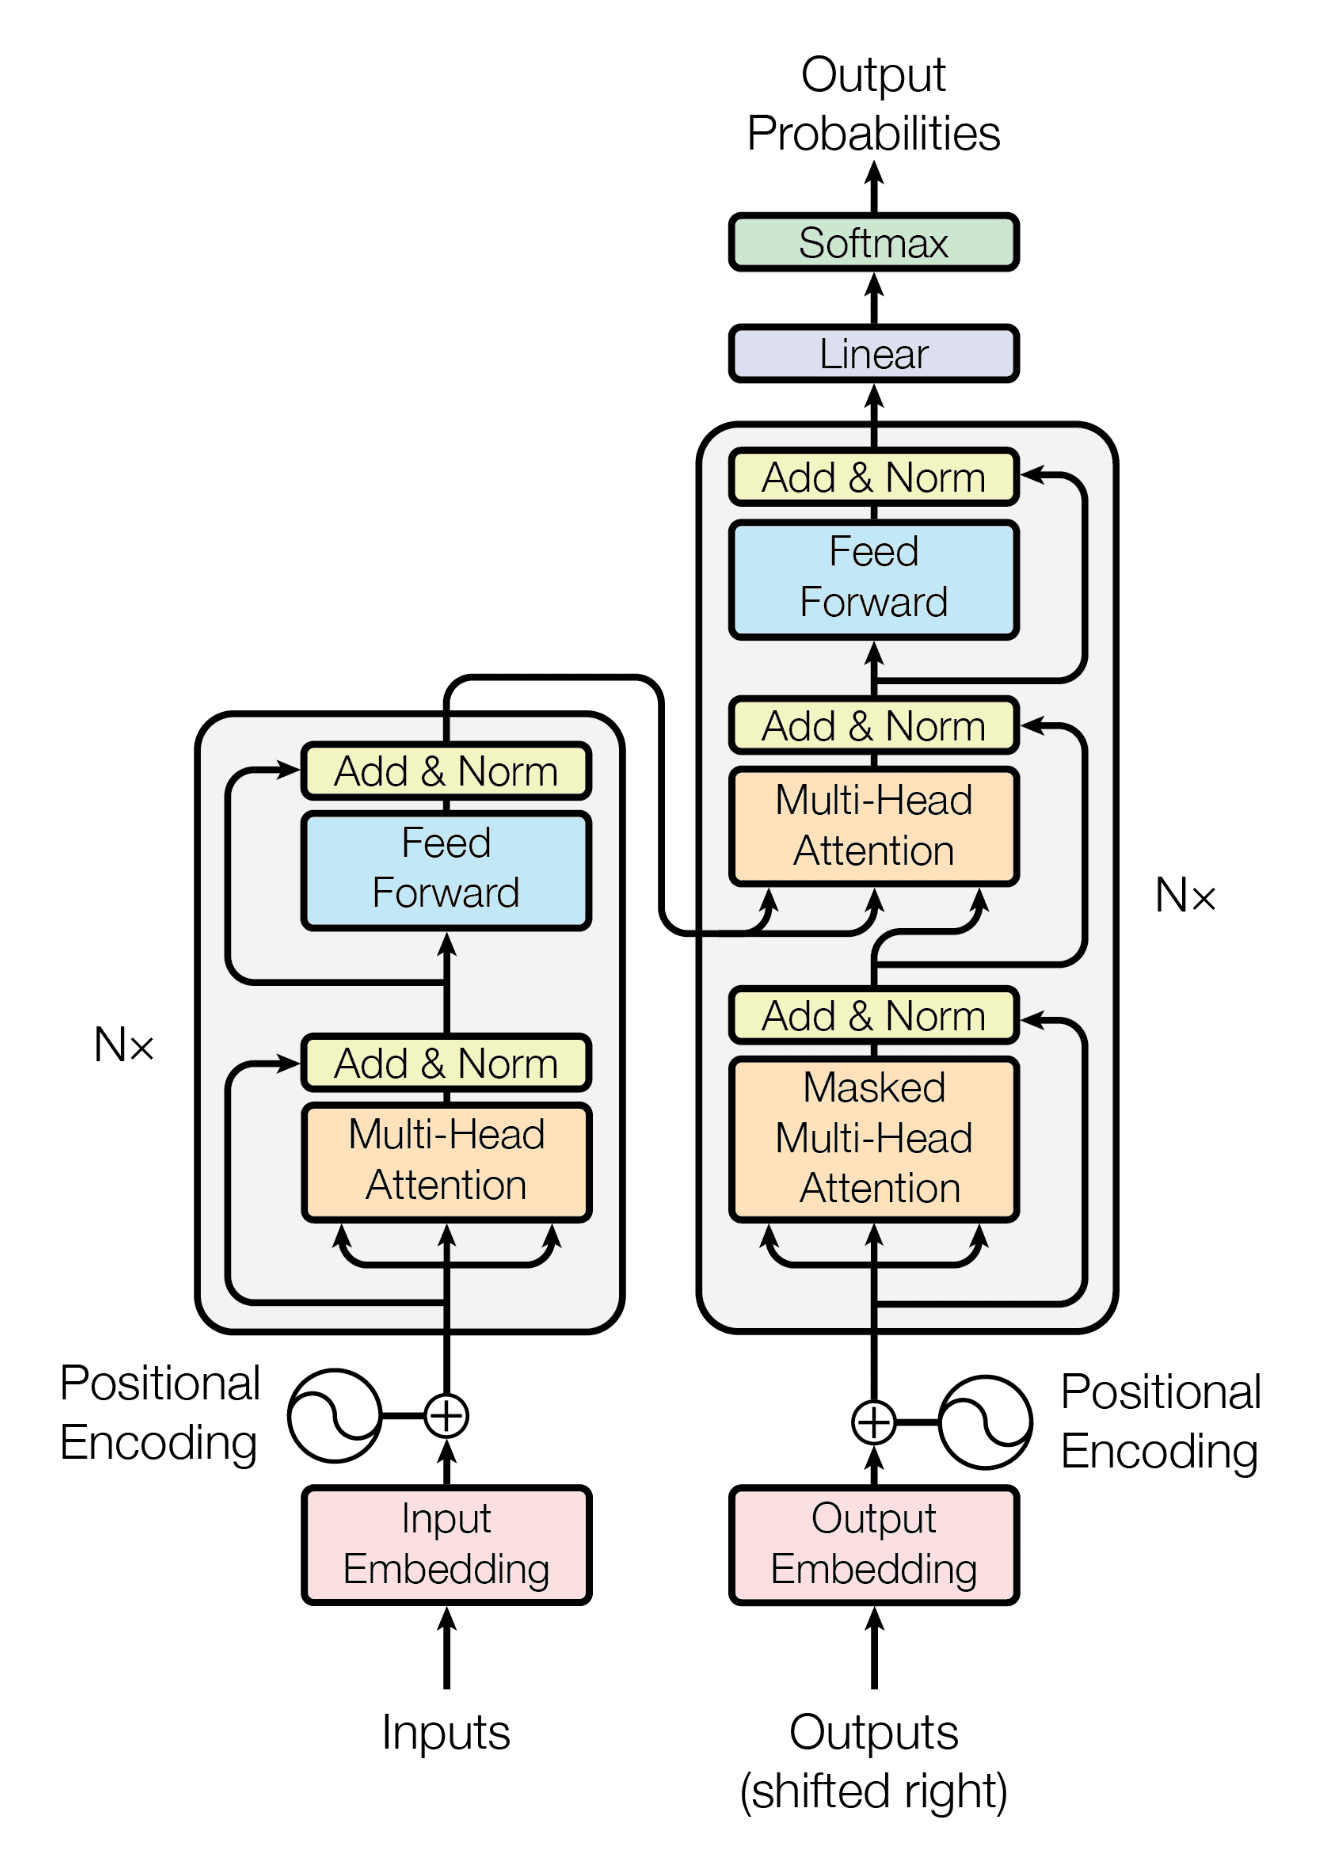
\includegraphics[width=0.5\textwidth]{figure/TransformerArch.png}
    \caption{La struttura Encoder-Decoder dell'architettura di un Transformer.}
    \label{fig:tranArch}
\end{figure}

\section{Problemi con RNN e CNN}
Nei capitoli precedenti abbiamo analizzato le reti convoluzionali e le reti ricorrenti, notando come riscontrassero delle criticità:
\begin{itemize}
    \item \textbf{RNN}: Esse processavano i dati sequenzialmente, vi era una problematica legata alla paralellizzazione dei processi, un altro problema aveva a che fare con la scomparsa/esplosione del gradiente su delle sequenze eccessivamente lunghe;
    \item \textbf{CNN}: Ottime per modelli locali, diventavano tuttavia molto inefficienti nel momento in cui si vuole catturare dipendenze molto lunghe, con la necessità pertanto di aumentarne la profondità.
\end{itemize}

Una delle soluzioni proposte è stata quella di usare il meccanismo dell'attenzione per modellare direttamente tutte le dipendenze in una singola sequenza, a prescindere dalla distanza, questa implementazione la ritroviamo nei Transformer.

\section{Visione ad alto livello}
A livello architetturale i Transformer si suddividono in due componenti principali:
\begin{itemize}
    \item \textbf{Encoder:} una pila di \textbf{N encoder} identici, nel paper in cui vengono presentati i Transformer ce ne sono 6, ognuno composto da due sottolivelli principali;
    \item \textbf{Decoder:} una pila di \textbf{N decoder} identici, anche in questo caso nel paper ce ne sono 6 specificando come il loro numero è strettamente collegato a quello degli encoder, anche i decoder, come gli encoder vengono strutturati in più sottolivelli.
\end{itemize}

Queste due componenti non condividono i pesi fra loro, analiziamo ora però i sottostrati degli Encoder, che sono fra loro indipendenti:

\begin{enumerate}
    \item \textbf{Self-Attention Layer:} consente all'encoder di "guardare" gli altri token presenti nella frase presa in input, mentre ne elabora uno nuovo per la parola presa in analisi;
    \item \textbf{Feed-Forward Neural Network:} l'output del self attention layer, viene passato a questo layer il quale applica indipendentemente le sue modifiche a ciascuna posizione del token di una frase.
\end{enumerate}

Il Decoder, oltre ad avere gli stessi due livelli presenti nell'Encoder, ne aggiunge uno ulteriore nel mezzo, chiamato \textbf{Encoder-Decoder Attention}, il quale si sofferma sulle parti più rilevanti della frase mandata in input.

\begin{figure}
    \centering
    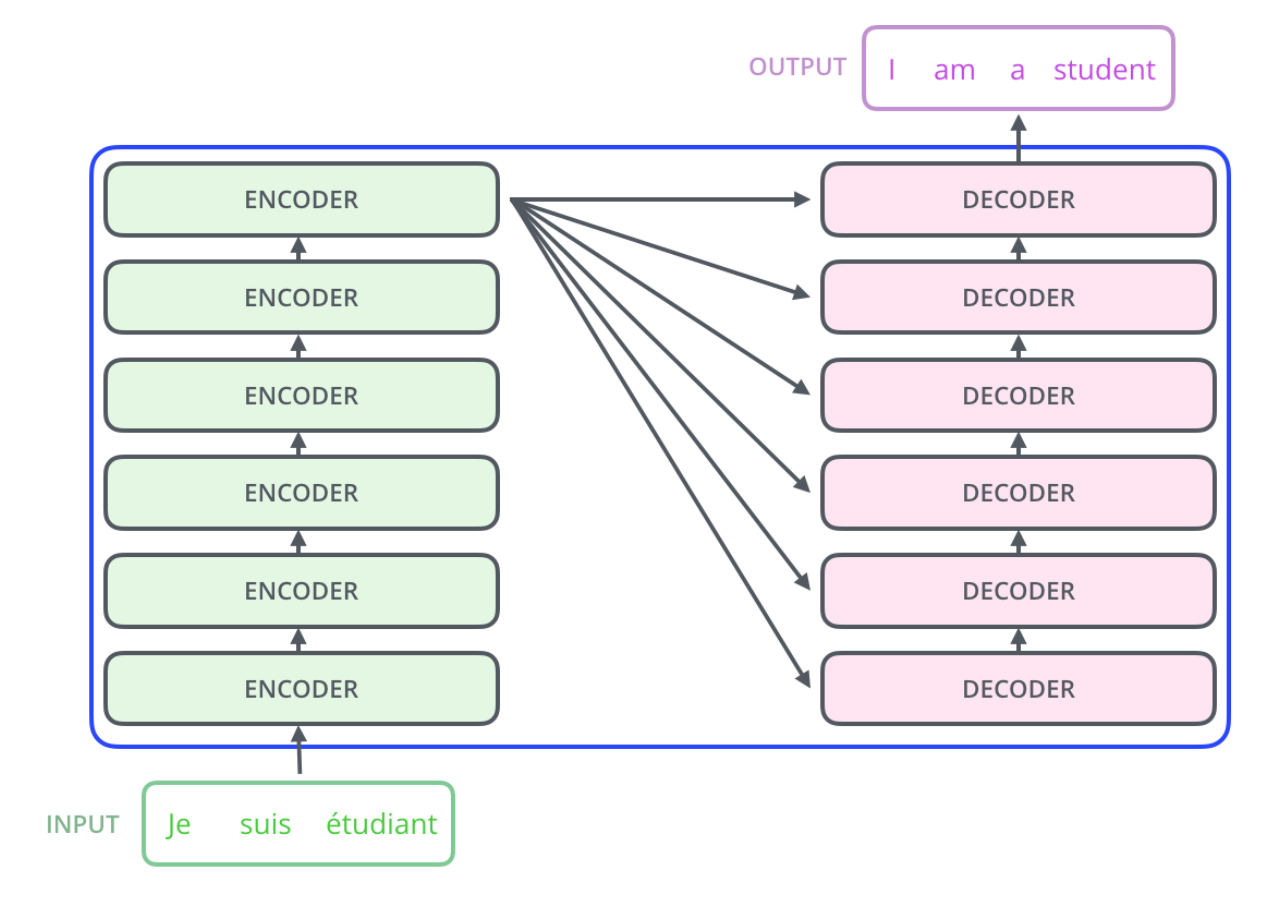
\includegraphics[width=\textwidth]{figure/EncDecTransformers}
    \caption{Rappresentazione ad alto livello di un'architettura di un Transformer, focalizzandosi principalmente sulla parte in cui vi sono gli Encoder e i Decoder}
    \label{fig:EncDecTrasf}
\end{figure}

\section{Introduzione ai Tensori}

Ogni parola data come input viene trasformata in un vettore di dimensione 512, tramite l'utilizzo di un algoritmo di embedding. La trasformazione in Embedding avviene solo nel primo Encoder. La lunghezza della frase, dunque il numero di vettori è un \textit{iperparametro}, il quale può essere impostato durante la progettazione. Una volta effettuato l'Embedding delle nostre parole, esse scorreranno all'interno dei vari layer presenti nei nostri Encoder. Ogni parola segue un suo percorso indipendente all'interno dell'Encoder, inoltre vengono create delle relazioni fra questi percorsi tramite il meccanismo dell'attenzione. Nel layer di feed-forward invece, non ci sono dipendenze e permettendo l'esecuzione parallela, aumentandone l'efficienza.

\section{Self-Attention}

Come già accennato in precedenza adesso, entriamo nel dettaglio per approfondire il \textit{Meccanismo dell'Attenzione}, questo meccanismo è l'effettiva rivoluzione che viene proposta da questa architettura~\cite{vaswani2017attention}, permettendo a ogni parola di ponderare la rilevanza della altre in una frase. Se consideriamo una frase con un soggetto sottointesto, per noi risulta semplice determinarne chi sia il soggetto, diversamente per una macchina questo risulta un meccanismo complesso. Questo problema viene arginato dal \textbf{Self-Attention Mechanism}, il quale collega i vari token presenti in una frase e determina le loro relazioni.

\begin{figure}
    \centering
    \includegraphics[width=0.65\textwidth]{figure/selfAttention}
    \caption{Nell'immagine possiamo vedere le singole relazioni, rappresentate dalle linee di connessione del token $\operatorname{it}\_$ con gli altri token della frase, più spessa è la linea, più solida risulta essere la relazione.}
    \label{fig:selfAtt}
\end{figure}


\subsection{Self-Attention in dettaglio}

La prima fase per il calcolo della \textbf{Self-Attention} comincia dalla creazione di tre vettori a partire da ogni vettore mandato in input agli Encoder. Vengono generati un vettore Query (Q), un vettore Key (K) e infine un vettore Value (V). La Self-Attention, si basa su una semplice idea: 

\begin{quote}
    \textit{Ogni parola (Query) cerca "parole chiavi" (Key), tra tutte le parole per capire da chi e quanta informazione prendere (Value).}
\end{quote}

Ogni token ha un Embedding, tutti questi vengono racchiusi in un vettore degli Embedding $E$, il quale viene moltiplicato per tre matici differenti: $W^Q$, $W^K$, $W^V$, tre matrici apprese durante il training, inizialmente inizializzate a valori piccoli le quali ci permettono di ottenere rispettivamente il Query vector, il Key vector e il Value vector.

\begin{equation}
    Q = E \times W^Q\,,\qquad K=E\times W^K\,,\qquad V=E\times W^V
\end{equation}
Una volta ottenuti i tre vettori 
$Q$, $K$ e $V$, si procede calcolando il grado di affinità tra ogni query $Q$ e tutte le chiavi $K$. Il risultato di questi confronti viene poi normalizzato dividendo per la radice quadrata della dimensione del vettore ($\sqrt{d_k}$). Una volta calcolati i tre vettori, effettuiamo dei confronti, in primis calcoliamo l'affinità fra ogni $Q$ con tutte le $K$, successivamente dividiamo per la radice quadrata del valore della dimensione di $Q$ e $K$, applichiamo la funzione $\operatorname{softmax}$ che ci dirà quanto sono compatibili. Infine moltiplichiamo tutto con i valori $V$, così il token corrente mixa informazioni dagli altri token in base all'attenzione.

\begin{equation}
    \operatorname{Attention}(Q,K,V) = \operatorname{softmax}\left(\frac{Q\,K^T}{\sqrt{d_k}}\right)\,V 
\end{equation}

\subsubsection{Esempio di calcolo}
Adesso prendiamo in analisi un esempio di calcolo partendo dalla seguente frase:
\begin{quote}
    Il gatto dorme.
\end{quote}

Ogni parola avrà un embedding corrispondente, immaginiamo in questo caso dei numeri molto semplici per facilità di comprensione:

\begin{table}[h!]
    \centering
    \caption{Embedding vettoriali delle parole}
    \begin{tabular}{@{}lc@{}}
        \toprule
        \textbf{Parola} & \textbf{Embedding} \\
        \midrule
        Il     & $\left[1, 0\right]$ \\
        Gatto  & $\left[0, 1\right]$ \\
        Dorme  & $\left[1, 1\right]$ \\
        \bottomrule
    \end{tabular}
\end{table}

Consideriamo le nostre matrici come delle matrici semplici, matrici identità, in modo tale che il prodotto fra matrici non sia eccessivamente complicato. Pertanto ottenendo i valori per ogni singola parola $Q,K,V$ saranno tutti la copia della singola parola presa in considerazione. Passo al confronto fra le singole parole, effettuando il prodotto scalare fra il vettore $Q$ e il vettore $K$ :

\begin{table}[!ht]
    \centering
    \caption{Prodotti scalari tra Query e Key per ogni coppia di parole}
    \begin{tabular}{@{}lccc@{}}
        \toprule
        \textbf{Da} & \textbf{Il ($[1, 0]$)} & \textbf{Gatto ($[0, 1]$)} & \textbf{Dorme ($[1, 1]$)} \\
        \midrule
        Il ($Q = [1, 0]$)     & 1 & 0 & 1 \\
        Gatto ($Q = [0, 1]$)  & 0 & 1 & 1 \\
        Dorme ($Q = [1, 1]$)  & 1 & 1 & 2 \\
        \bottomrule
    \end{tabular}
\end{table}

Effettuando questi prodotti scalari, dividerò i singoli valori per la radice quadrata della grandezza dei vettori, nel nostro caso per $\sqrt{2}$ per poi sottoporli a una \textbf{softmax}, la quale ci darà dei pesi, che sommati, ci daranno un valore unitario. Essa enfatizzerà l'importanza delle parole più rilevanti, rendendo il modello capace di contestualizzare correttamente ogni termine.

\subsubsection{L'analogia delle cartelle}
Supponiamo di avere un armadietto, al quale interno ci sono numerose cartelle, il nostro obbiettivo è trovare la cartella corrispondente al post-it che abbiamo in mano (Figura~\ref{fig:folderAn}). Il post-it è la nostra query, le key è l'identificativo della nostra cartella, dunque il loro nome. Una volta che trovo una corrispondenza fra la cartella e il post-it, prendiamo la cartella e la poniamo al di fuori del nostro armadietto, aprendola al suo interno abbiamo dei documenti che sono il value. Moltiplicare il vettore query per ogni vettore chiave produce un punteggio per ogni cartella, il quale punteggio maggiore mette in evidenza la corrispondenza più quotata fra le due parole.

\begin{figure}[hbtp]
    \centering
    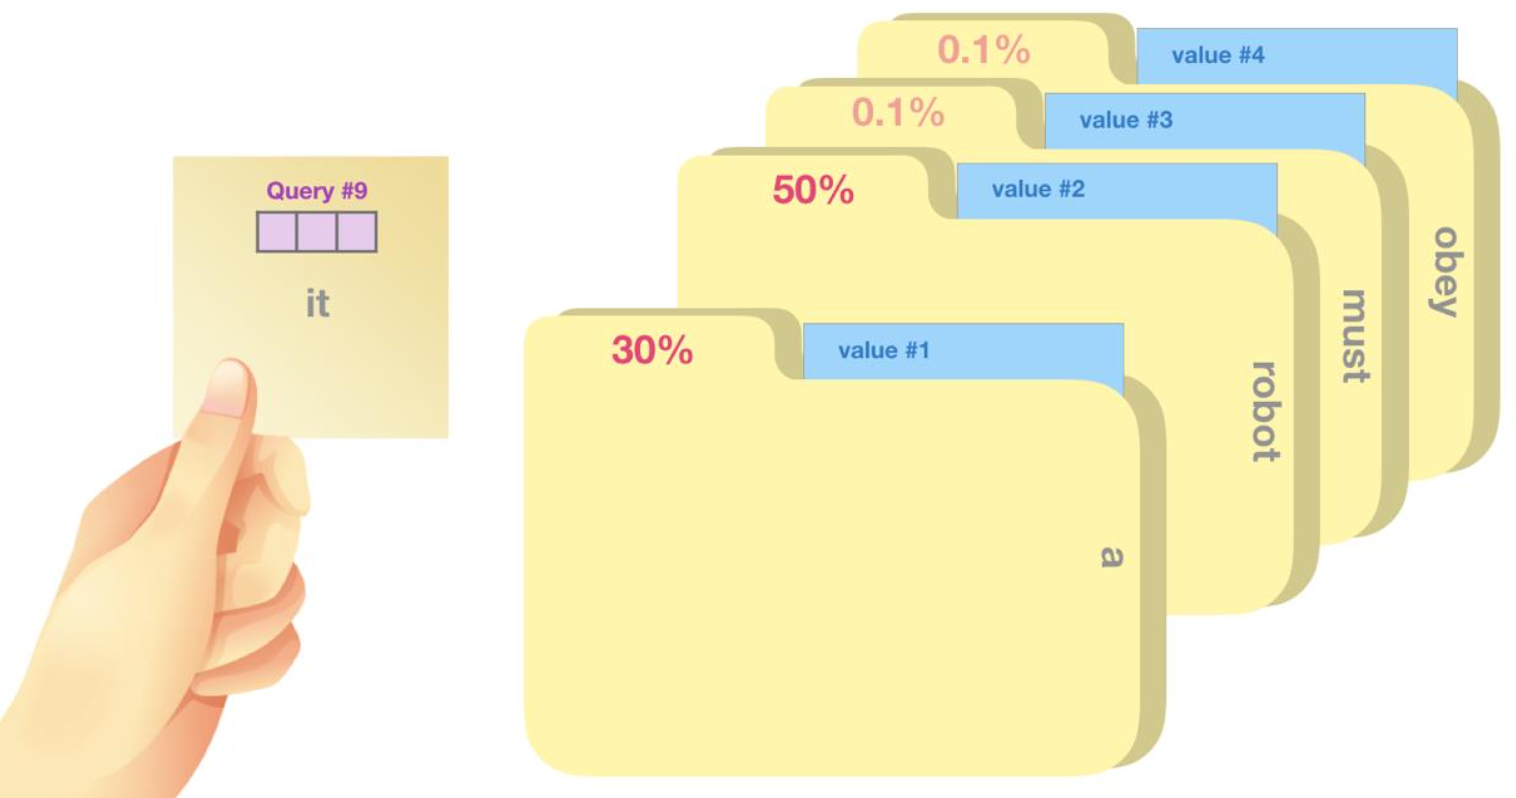
\includegraphics[width=0.75\textwidth]{figure/FoldeAnalogy.png}
    \caption{Rappresentazione dell'analogia delle cartelle, nel quale si rappresentano i tre vettori, query vector come il post-it, key vector come l'identificativo di ogni cartella, value vector come il valore all'interno di ogni cartella, ogni cartella ha un punteggio che mappa la percentuale di corrispondenza.}
    \label{fig:folderAn}
\end{figure}

\section{Multi-Head Attention}

Il meccanismo di Self-Attention può essere raffinato tramite l'introduzione della \textbf{Multi-Head Attention}, una tecnica che migliora l'efficacia dell'attenzione secondo due principali direttrici:

\begin{enumerate}
    \item Amplia la capacità del modello di focalizzarsi su posizioni differenti nella sequenza di input. Ad esempio, il vettore $z_1$ associato alla prima parola potrebbe rappresentare un misto di tutte le codifiche, ma al contempo essere fortemente influenzato dalla parola stessa;
    \item Introduce molteplici \textit{sottospazi di rappresentazione} all'interno dello stesso livello di attenzione. Invece di utilizzare un singolo insieme di matrici di peso per $Q$, $K$ e $V$, si impiegano più insiemi distinti, ciascuno inizializzato in modo indipendente. Al termine dell’addestramento, ogni insieme proietta gli embedding d’ingresso in uno spazio latente diverso, catturando così vari aspetti delle relazioni tra parole.
\end{enumerate}

Questo meccanismo introduce diverse \textbf{Teste di Attenzione} (\textit{Heads}), ognuna delle quali applica il calcolo di attenzione in modo indipendente, utilizzando parametri distinti. Ogni testa analizza l’input da una prospettiva differente, permettendo al modello di cogliere vari tipi di relazioni semantiche e sintattiche tra le parole. Alla fine, i vettori prodotti da ciascuna testa ($z_i$) vengono concatenati e successivamente proiettati in uno spazio comune tramite una matrice di pesi addizionale, $W_o$, appresa durante l’addestramento. Questo passaggio ha lo scopo di restituire un singolo vettore di output da fornire al livello Feed-Forward della rete.

\subsubsection{Esempio}

Consideriamo nuovamente una frase semplice per illustrare il funzionamento:

\begin{quote}
Il gatto che inseguiva il topo miagolava.
\end{quote}

Focalizziamoci sulla parola \textit{miagolava}. Essa intrattiene relazioni diverse con le parole precedenti: \textit{gatto} è il soggetto che compie l’azione, \textit{inseguiva} rappresenta un’azione precedente, mentre \textit{topo} non ha relazione semantica diretta con l’azione del miagolare. Una singola testa di attenzione faticherebbe a modellare contemporaneamente tutte queste relazioni, per questo la Multi-Head Attention risolve questo problema. Dal punto di vista grafico, ciò rende la rappresentazione visiva del meccanismo più complessa rispetto al caso della Self-Attention classica (Figura~\ref{fig:selfAtt}), ma allo stesso tempo più espressiva e potente (Figura~\ref{fig:multiHeadAtt}).

\begin{figure}
    \centering
    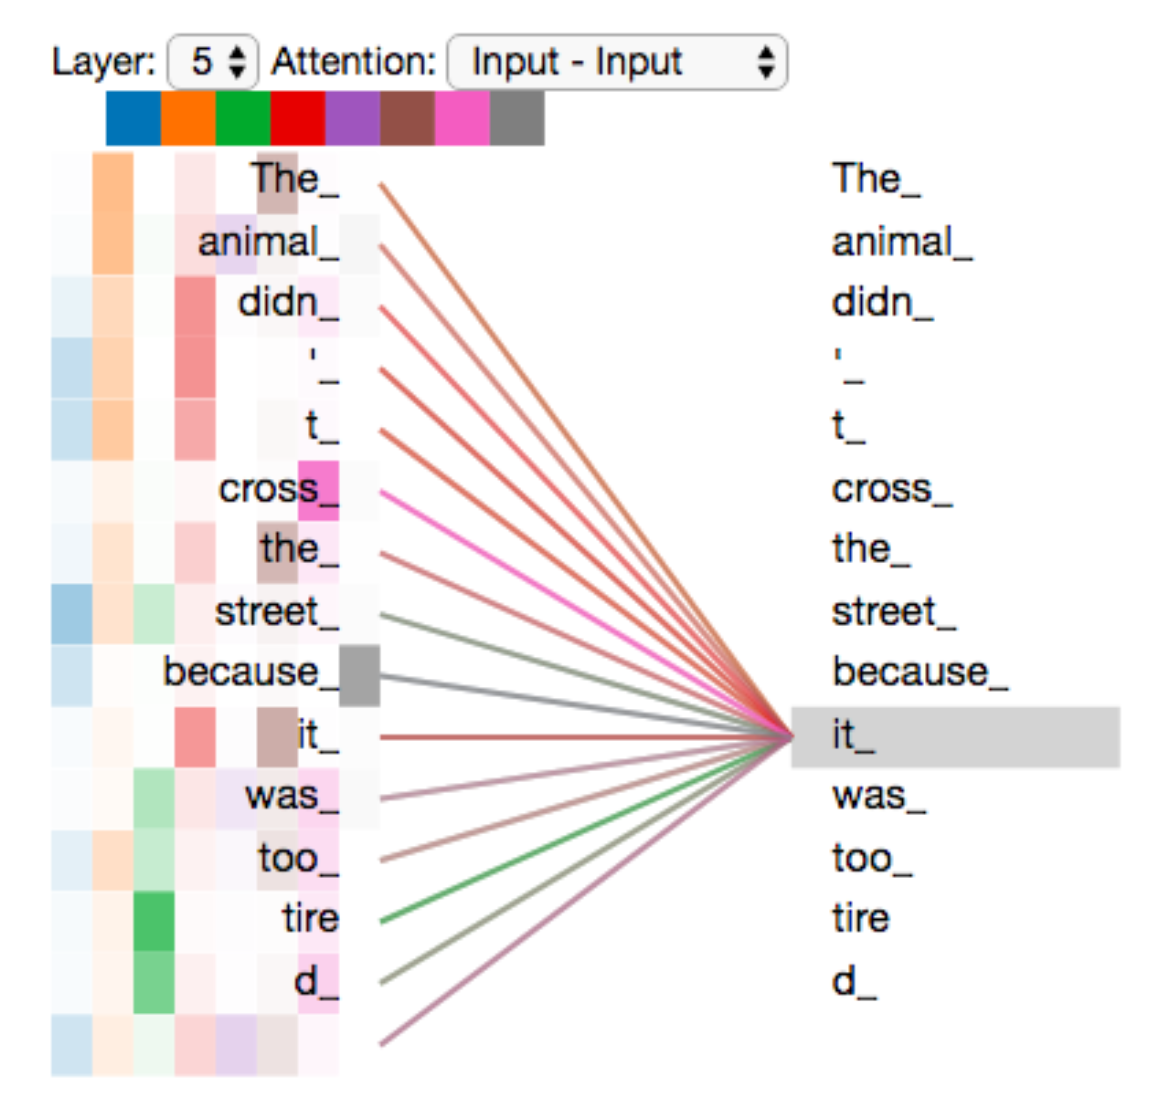
\includegraphics[width=0.5\textwidth]{figure/MultiHeadAttention}
    \caption{Esempio visivo della Multi-Head Attention: ogni testa stabilisce relazioni differenti tra la parola "it" e le altre nel contesto, evidenziate con colori distinti.}
    \label{fig:multiHeadAtt}
\end{figure}

\section{Positional Encoding}

Una limitazione intrinseca del meccanismo di \textit{Self-Attention} è la mancanza di una nozione di ordine all'interno della sequenza.  
A differenza delle reti ricorrenti, i Transformer elaborano tutti i token in parallelo, senza alcuna informazione sulla loro posizione nella frase. Questo significa che, senza un intervento aggiuntivo, il modello non sarebbe in grado di distinguere tra frasi come "il cane morde l’uomo" e "l’uomo morde il cane". Per ovviare a questo problema, i Transformer introducono un meccanismo chiamato \textbf{Positional Encoding}. L’idea è semplice ma potente: ad ogni embedding di input si aggiunge un \textit{vettore di posizione}, che codifica la posizione del token nella sequenza. In questo modo, il modello acquisisce un "senso dell’ordine" necessario per comprendere la struttura sintattica e semantica delle frasi. A differenza degli altri parametri del modello, questi vettori non vengono appresi durante l’addestramento, ma sono definiti in modo deterministico secondo un pattern \textbf{Sinusoidale}. La loro costruzione è tale da garantire che le differenze tra posizioni risultino ancora percepibili dopo la proiezione nei vettori $Q$, $K$ e $V$, influenzando così il calcolo dell’attenzione. I vettori di Positional Encoding sono definiti dalle seguenti funzioni periodiche:

\begin{equation}
PE_{(\operatorname{pos},2i)} = \sin\left(\frac{\operatorname{pos}}{10000^{\frac{2i}{d_{\operatorname{model}}}}}\right), \quad
PE_{(\operatorname{pos},2i+1)} = \cos\left(\frac{\operatorname{pos}}{10000^{\frac{2i}{d_{\operatorname{model}}}}}\right)
\end{equation}

dove:
\begin{itemize}
    \item $\operatorname{pos}$ è la posizione del token nella sequenza;
    \item $i$ rappresenta l’indice della dimensione dell’embedding;
    \item $d_{\operatorname{model}}$ indica la dimensione totale dell’embedding del modello.
\end{itemize}

Ogni dimensione dell’embedding segue un’onda sinusoidale con frequenza diversa. Le frequenze crescono in modo geometrico: alcune onde variano lentamente (rappresentano la posizione su larga scala), altre variano rapidamente (catturano differenze locali tra parole vicine). Questa combinazione consente di rappresentare in modo univoco e continuo ogni posizione nella sequenza. Un aspetto notevole di questa scelta progettuale è che le posizioni relative possono essere descritte in modo lineare: dato un offset $k$, il Positional Encoding della posizione $\operatorname{pos} + k$ può essere espresso come una funzione lineare di quello in $\operatorname{pos}$. Ciò facilita il compito del modello nel riconoscere distanze e relazioni relative tra i token, indipendentemente dalla loro posizione assoluta.
\begin{figure}[hbtp]
    \centering
    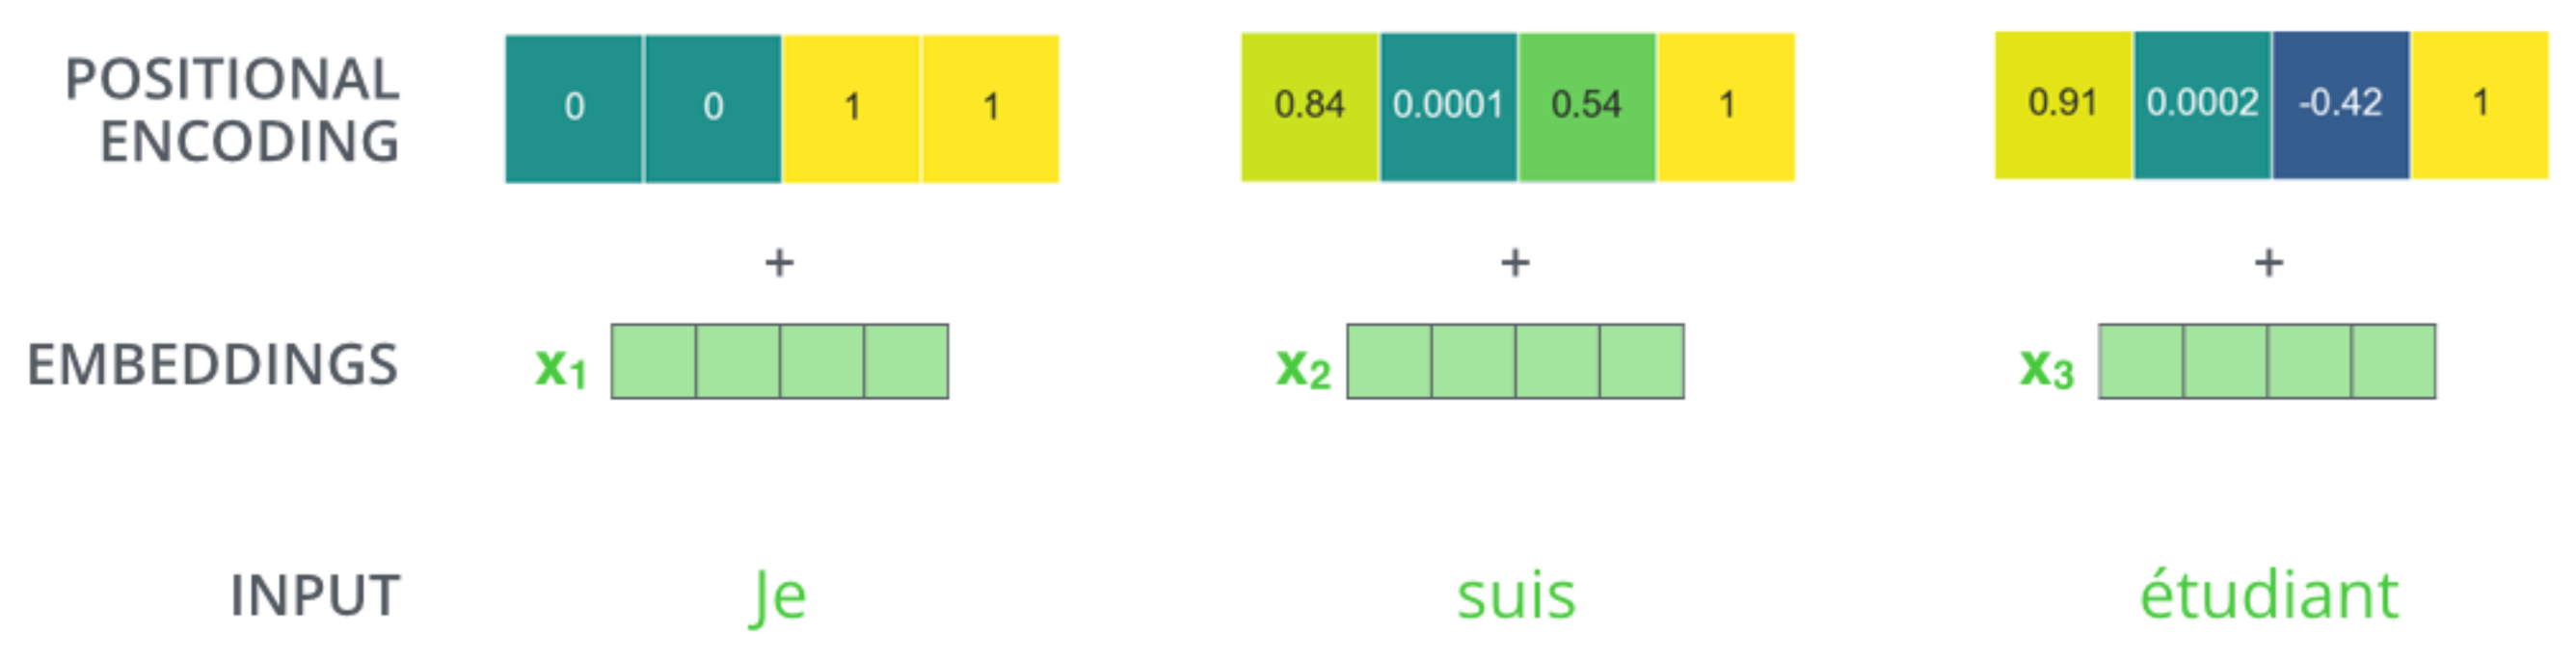
\includegraphics[width=0.85\textwidth]{figure/PositionalEncoding}
    \caption{Esempio di combinazione tra gli embedding delle parole e i vettori di Positional Encoding. Ogni token dell’input viene rappresentato dal proprio embedding lessicale, al quale viene sommato un vettore di Positional Encoding. Quest’ultimo fornisce al modello l’informazione sulla posizione relativa del token nella sequenza, consentendo al Transformer di distinguere l’ordine delle parole pur elaborandole in parallelo.}
    \label{fig:posEncoding}
\end{figure}
Gli esperimenti condotti nel lavoro originale~\cite{vaswani2017attention} hanno mostrato che questo schema sinusoidale è efficace quanto i Positional Encoding appresi, con il vantaggio di non introdurre ulteriori parametri da ottimizzare durante l’addestramento.

\section{Residual Connections}

Un altro elemento dell’architettura Transformer è rappresentato dalle \textbf{Connessioni Residue} (\textit{Residual Connections}). Queste connessioni sono nate con le reti \textit{ResNet} e hanno rivoluzionato il modo in cui vengono addestrate le reti neurali profonde, permettendo di preservare il flusso dell’informazione e rendendo l’ottimizzazione più stabile. L’idea alla base è semplice ma estremamente efficace: invece di far passare l’input attraverso una lunga catena di trasformazioni che rischiano di distorcere o attenuare il segnale, si consente all’informazione originale di "saltare" direttamente uno o più strati. Formalmente, se uno strato applica una trasformazione $F(x)$ al suo input $x$, l’uscita dello strato diventa:

\begin{equation}
    \operatorname{Output} = F(x) + x
\end{equation}

In altre parole, il risultato finale non è solo la trasformazione $F(x)$, ma una combinazione dell’input originale e della sua versione modificata. Questo semplice schema consente al modello di apprendere più facilmente funzioni identitarie (cioè $F(x) \approx 0$), riducendo il rischio che l’informazione iniziale venga "dimenticata" nei livelli successivi. All’interno del Transformer, ogni blocco, sia nell’encoder che nel decoder, utilizza questo principio attraverso una struttura chiamata \textbf{Add \& Norm}.  
Ogni sottoblocco (che può essere un modulo di \textit{Multi-Head Attention} o un livello \textit{Feed-Forward}) è avvolto da questa componente, che:
\begin{enumerate}
    \item Somma l’input del blocco con la sua uscita trasformata (connessione residua);
    \item Normalizza il risultato tramite una \textit{Layer Normalization}.
\end{enumerate}

\begin{figure}[hbtp]
    \centering
    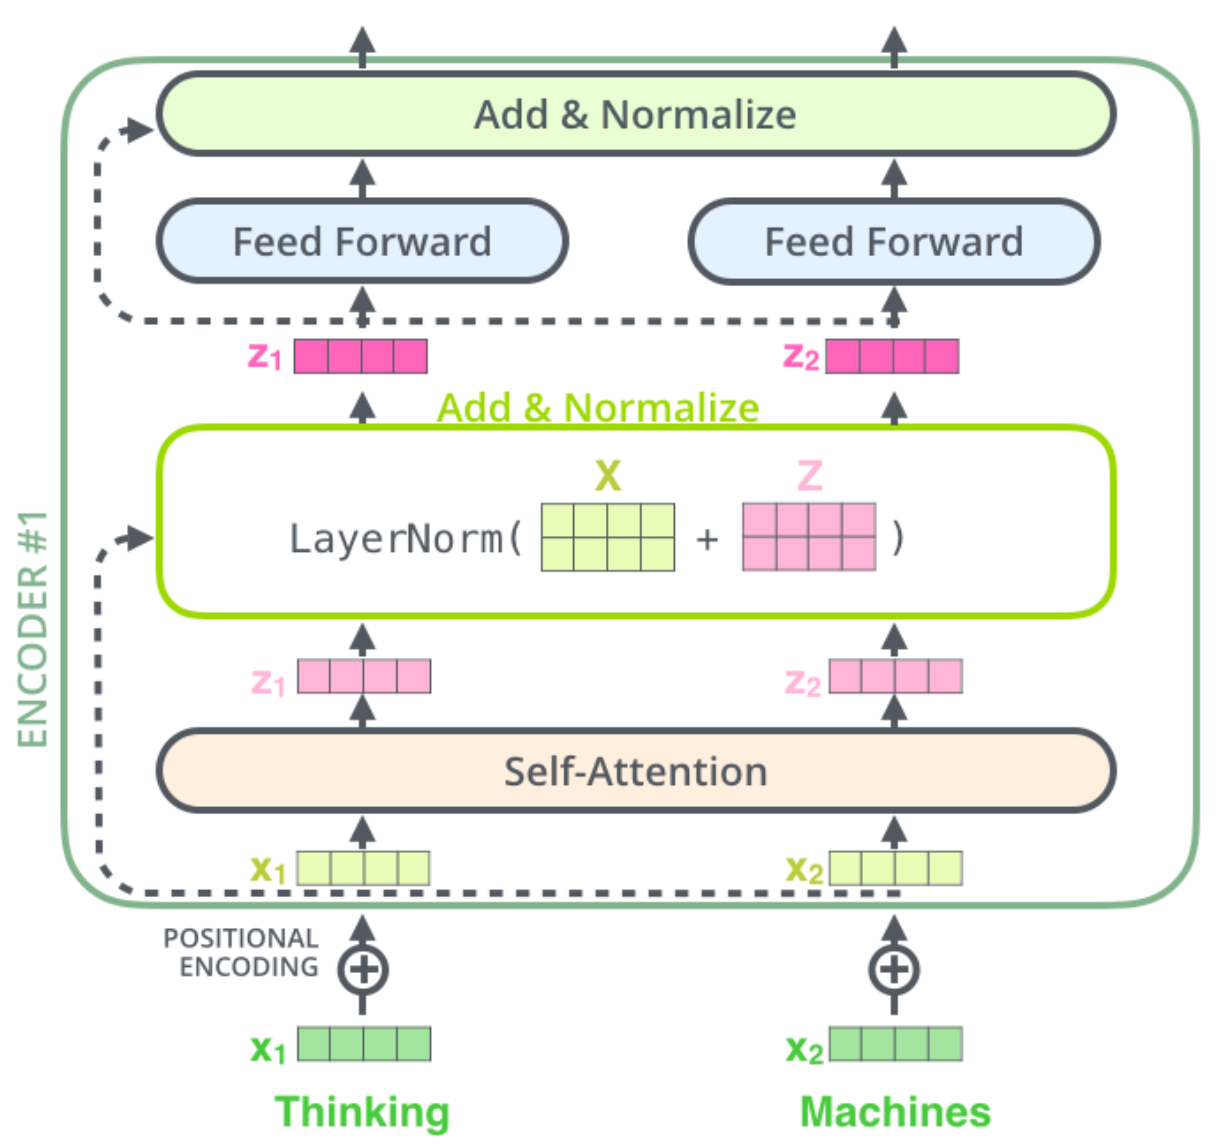
\includegraphics[width=0.6\textwidth]{figure/ResidualAddon.png}
    \caption{Struttura del blocco \textit{Add \& Norm}, che combina una connessione residua con la normalizzazione per mantenere la stabilità numerica e il flusso informativo.}
    \label{fig:ResAddon}
\end{figure}
Le connessioni residue portano diversi vantaggi chiave:
\begin{itemize}
    \item \textbf{Mitigazione del problema del gradiente che scompare:} agevolano la retropropagazione del gradiente anche in reti molto profonde, migliorando la stabilità dell’addestramento;
    \item \textbf{Preservazione dell’informazione originale:} permettono al modello di conservare parti essenziali dell’input che potrebbero essere degradate dalle trasformazioni non lineari successive;
    \item \textbf{Facilitazione dell’apprendimento:} rendono più semplice apprendere trasformazioni che si discostano poco dall’identità, accelerando la convergenza.
\end{itemize}
In termini intuitivi, le connessioni residue possono essere viste come una sorta di \textbf{corsia preferenziale per l’informazione}. Il modello può decidere, in ogni blocco, se utilizzare il segnale trasformato, mantenere quello originale o combinare entrambi. Questo meccanismo diventa particolarmente prezioso in architetture molto profonde, dove l’accumulo di trasformazioni rischierebbe di attenuare o distorcere il contenuto semantico iniziale, compromettendo la coerenza dell’apprendimento.

\section{Decoder}

Il \textbf{Decoder} invece, ha il compito di generare la sequenza di output a partire dalla rappresentazione codificata dell’input, fornita dall’Encoder. In particolare, l’output dell’ultimo strato dello stack degli Encoder viene trasformato in un insieme di vettori chiave ($K$) e valore ($V$), i quali saranno utilizzati in ogni strato del decoder all’interno del modulo \textit{Encoder-Decoder Attention}. Questo meccanismo permette al Decoder di concentrarsi su specifiche porzioni della sequenza di input, fornendo così una forma di allineamento tra input e output. Il processo si ripete finché non viene generato un simbolo speciale di fine sequenza (\texttt{<eos>}), che segnala al modello il termine della generazione. Ad ogni passo, l’output prodotto dal Decoder viene reinserito come input per il passo successivo, e tale operazione prosegue lungo la pila di Decoder in maniera analoga a quanto accade per l’Encoder. Anche nel Decoder, viene incorporata l’informazione posizionale, attraverso apposite rappresentazioni, per permettere al modello di distinguere l’ordine delle parole nella sequenza.
\begin{figure}
    \centering
    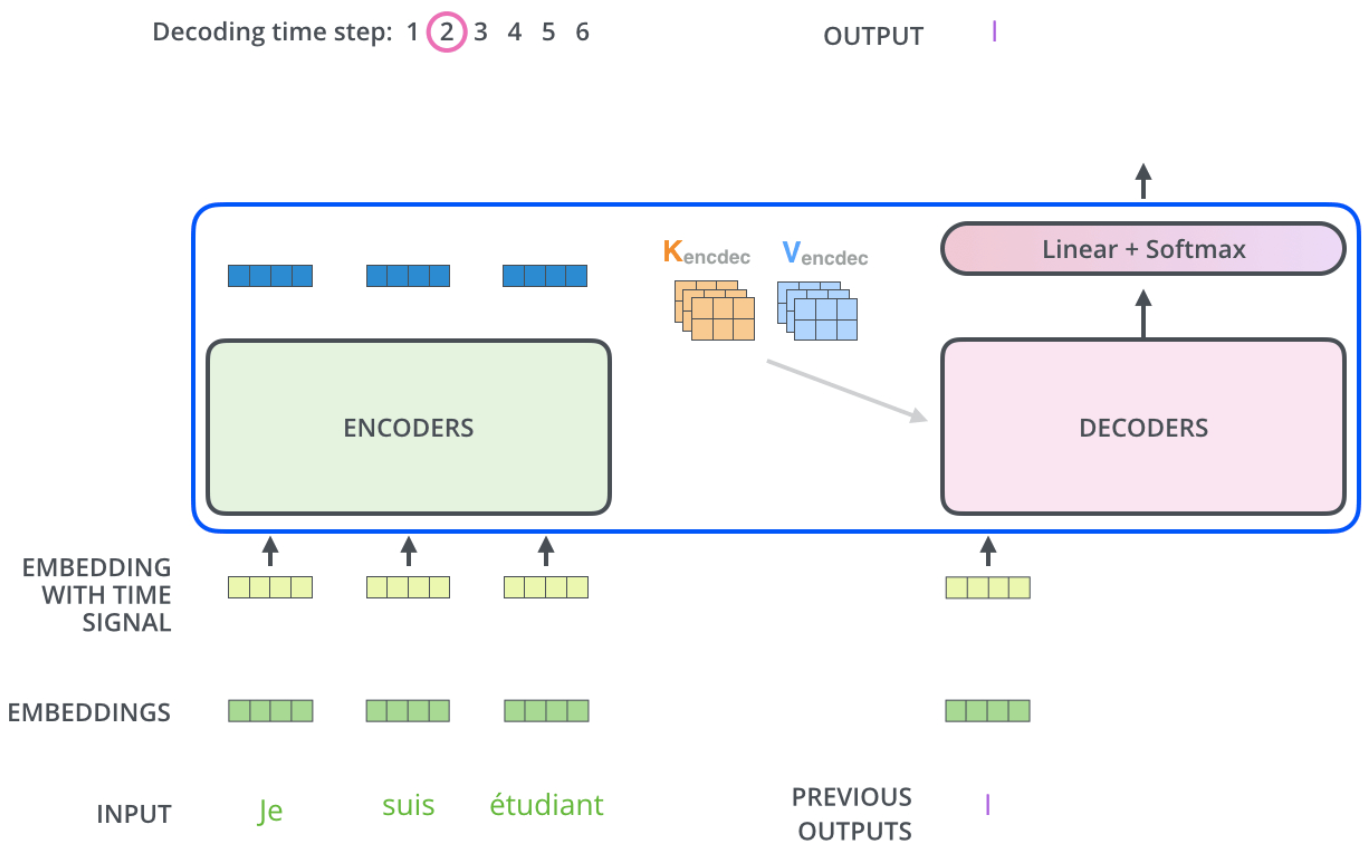
\includegraphics[width=0.9\textwidth]{figure/DecoderSample.png}
    \caption{Esempio del processo di generazione nel decoder al secondo step temporale. Nel primo step è stata generata la parola \textit{I} come traduzione di \textit{je}.}
    \label{fig:DecSam}
\end{figure}
Riseptto all’Encoder nel meccanismo di \textbf{Self-Attention} impiegato nel Decoder c'è una differenza. L’attenzione viene \textit{mascherata} per evitare che il modello acceda a posizioni future della sequenza di output. Precisamente, alle posizioni successive viene assegnato il valore $-\infty$ prima dell'applicazione della funzione $\operatorname{softmax}$, così da annullarne il contributo. Il modulo \textit{Encoder-Decoder Attention}, invece, opera in maniera analoga alla Self-Attention Multi-Head, con la differenza che le matrici $K$ e $V$ provengono direttamente dall’output dello stack degli Encoder, mentre le matrici $Q$ (Query) vengono calcolate a partire dallo strato sottostante del Decoder stesso.

\subsection{Final Layer e Softmax}

Lo stack dei Decoder, al termine della generazione, produce un vettore continuo (un vettore di float), che deve essere convertito in una parola del vocabolario. A questo scopo intervengono due componenti finali: il \textbf{Final Linear Layer} e il \textbf{Softmax Layer}. Il \textit{Final Linear Layer} è una rete completamente connessa che trasforma il vettore di rappresentazione generato dal decoder in un \textbf{vettore di logit} ossia dati grezzi. Questo vettore ha una dimensione pari alla cardinalità del vocabolario: ad esempio, se il modello gestisce un vocabolario di 10.000 parole, il vettore sarà lungo 10.000, e ciascun valore rappresenterà il punteggio non normalizzato associato a una specifica parola. Il \textit{Softmax Layer} converte questo vettore di logit in una distribuzione di probabilità: tutti i valori risultanti saranno positivi e la loro somma sarà pari a uno. L’indice con la probabilità più alta indicherà la parola da generare in quello specifico time step.

\begin{figure}
    \centering
    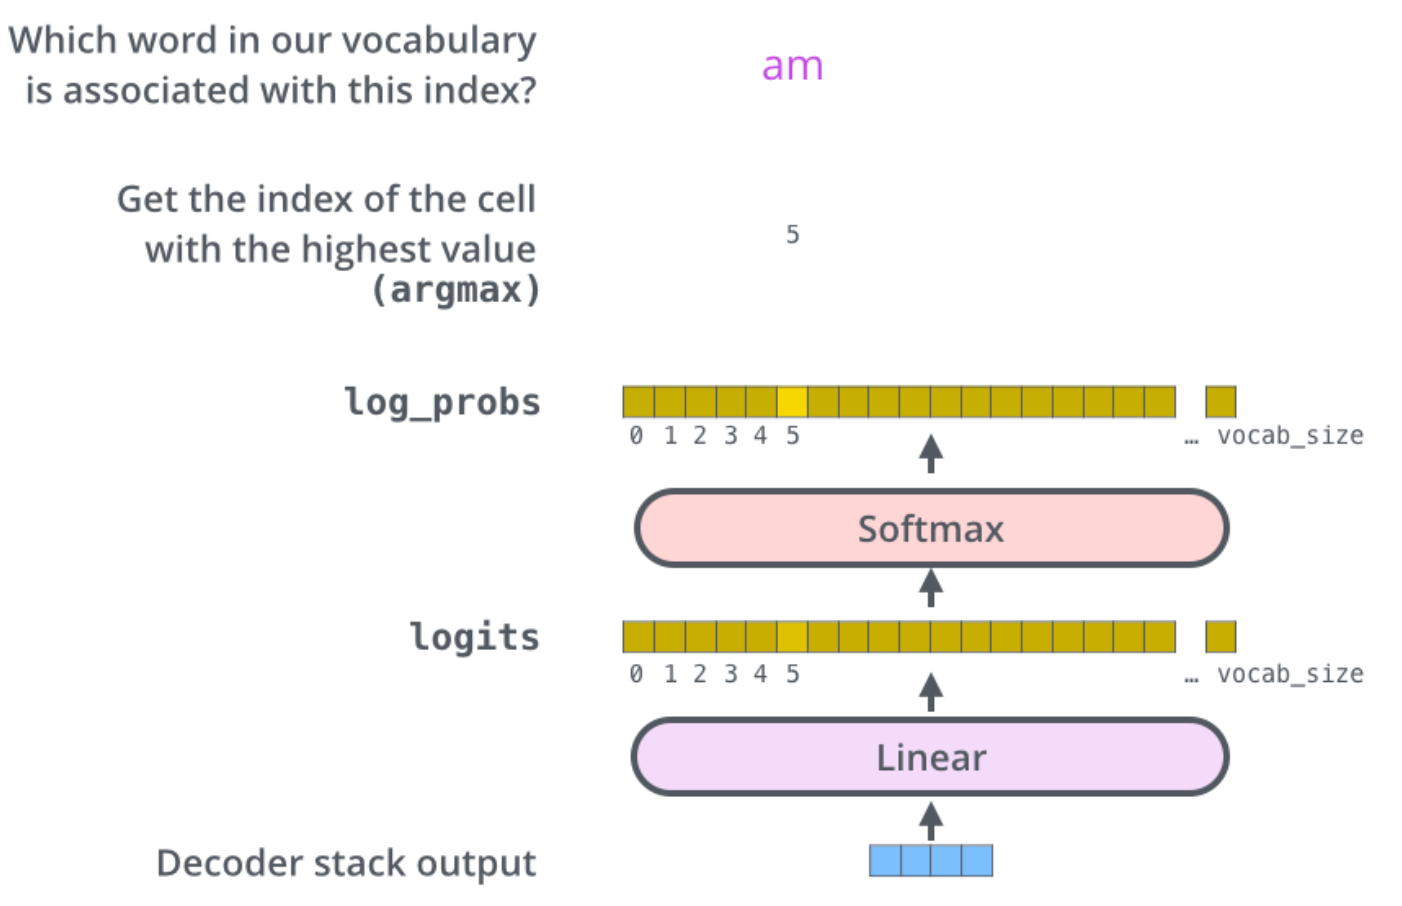
\includegraphics[width=0.75\textwidth]{figure/FinalLayer.png}
    \caption{Struttura dei layer finali del decoder nel Transformer, che trasformano la rappresentazione vettoriale in una parola.}
    \label{fig:FinLay}
\end{figure}

\section{Allenamento di un Transformer}

Durante la fase di \textbf{training}, il Transformer esegue un \textit{forward pass} sui dati forniti. Poiché il dataset di training è etichettato, è possibile confrontare le uscite del modello con i target attesi, valutando così la qualità delle predizioni. In presenza di discrepanze tra output previsto e desiderato, si procede con un aggiornamento dei pesi tramite backpropagation, al fine di minimizzare l’errore. I vocabolari utilizzati nei Transformer contengono generalmente un numero elevato di parole, oltre a simboli speciali. Prima del training, ogni parola viene mappata su un vettore numerico tramite un processo di \textit{preprocessing}. Una rappresentazione comune è la \textbf{One-Hot Encoding}, in cui ogni parola, è rappresentata da un vettore con tutti zeri, tranne un valore pari a uno in corrispondenza della posizione associata alla parola nel vocabolario. Nelle prime fasi di training, un modello non ancora addestrato produce uscite casuali e scorrelate dal target. L’obiettivo del training è dunque quello di guidare il modello a produrre, per ciascun time step, una distribuzione di probabilità in cui la parola attesa abbia la probabilità più alta. In particolare, ci si aspetta che la prima distribuzione assegni il valore di probabilità più alto alla prima parola desiderata, la seconda alla seconda parola, e così via, fino all’ultima distribuzione, in cui la probabilità più alta dovrebbe corrispondere al token \texttt{<eos>}, segnalando la fine della sequenza.

\begin{figure}
    \centering
    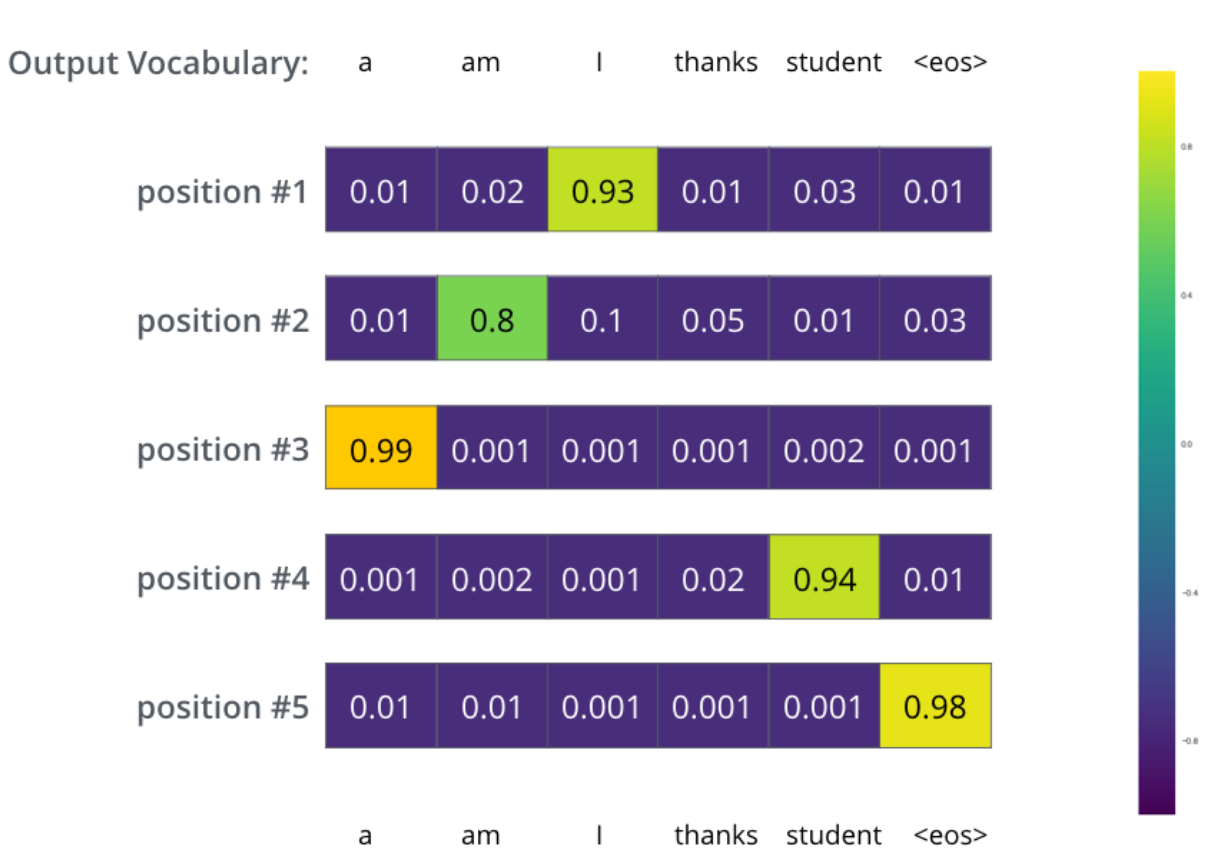
\includegraphics[width=0.7\textwidth]{figure/TrainExpectation}
    \caption{Distribuzioni di probabilità prodotte dal decoder: ogni posizione temporale è associata a una distribuzione su tutto il vocabolario, e ci si aspetta che la parola target sia quella con la probabilità massima.}
    \label{fig:trainExp}
\end{figure}

\section{Oltre la struttura del Transformer}

Con la comprensione completa dell'architettura originaria del Transformer, siamo ora pronti ad analizzare alcune delle estensioni che hanno reso questo modello uno standard de facto nel campo del Deep Learning. In particolare, approfondiremo come il Transformer venga adattato a contesti specifici mediante il \textbf{fine-tuning}, quali siano le sue principali \textbf{applicazioni} in scenari reali e accademici, e infine esamineremo alcune delle \textbf{varianti architetturali} che ne estendono le potenzialità, spesso superandone i limiti originali.

\section{Fine-Tuning del Transformer}

Il \textbf{Fine-Tuning} è una tecnica di apprendimento trasferito (\textit{transfer learning}) ampiamente adottata nel contesto dei Transformer, che consente di adattare un modello pre-addestrato a un compito specifico. Il modello viene inizialmente addestrato su un vasto corpus general-purpose (come Wikipedia o Common Crawl), apprendendo rappresentazioni linguistiche ricche e versatili. Successivamente, viene ottimizzato su un dataset mirato, spesso molto più piccolo, relativo a un task specifico (e.g Sentiment Analysis, Entity Recognition, Code Generation, ecc\ldots). Il processo si articola come segue:
    \begin{enumerate}
        \item \textbf{Pretraining:} il modello viene addestrato in maniera auto-supervisionata su un task generale;
        \item \textbf{Fine-tuning supervisionato:} si sostituisce o si estende la testa del modello con uno o più layer adatti al task target, e si effettua un training supervisionato con gradient descent.
    \end{enumerate}
Uno degli aspetti cruciali del fine-tuning è la scelta del \textit{Learning Rate}: un tasso troppo elevato potrebbe sovrascrivere le rappresentazioni apprese nel pretraining; al contrario, uno troppo basso potrebbe non fornire l'adattamento desiderato. Il fine-tuning può essere visto come l’aggiustamento delicato di migliaia (o miliardi) di piccole manopole, ovvero i parametri del modello, che sono già stati impostati in una configurazione utile durante la fase di pre-addestramento. Durante il fine-tuning, queste manopole non vengono azzerate né completamente ricalibrate, ma solo ritoccate per adattare il modello a un nuovo compito specifico. In questo modo, si parte da una conoscenza generale già appresa e la si "rifinisce", ottenendo una configurazione dei parametri più adatta al contesto desiderato.

\section{Applicazioni del Transformer}

L'architettura Transformer è stata adottata in una vasta gamma di applicazioni, sia in ambito linguistico che in domini non testuali. Tra le principali possiamo trovare:

\begin{itemize}
    \item \textbf{Natural Language Processing (NLP):} è il dominio originario del Transformer, dove viene impiegato in:
    \begin{itemize}
        \item Traduzione automatica (e.g. Google Translate);
        \item Generazione di testo (e.g. ChatGPT, GPT-5);
        \item Sentiment Analysis;
        \item Named Entity Recognition (NER);
        \item Riassunto automatico.
    \end{itemize}
    \item \textbf{Visione artificiale (CV):} con modelli come Vision Transformer (ViT), l'architettura viene adattata al dominio visivo per compiti come classificazione, segmentazione e object detection;
    \item \textbf{Bioinformatica e Chimica Computazionale:} i Transformer vengono utilizzati per la modellazione di sequenze proteiche, il drug discovery, e la predizione di interazioni molecolari;
    \item \textbf{Codice e programmazione automatica:} modelli come Codex e CodeBERT sfruttano il Transformer per comprendere e generare codice sorgente;
    \item \textbf{Musica, immagini e altre modalità:} modelli come MuseNet o DALL-E impiegano architetture Transformer per generare musica e immagini, integrando capacità multi-modali.
\end{itemize}

\section{Varianti dell'Architettura Transformer}

L'efficacia e la flessibilità del Transformer hanno portato allo sviluppo di numerose varianti architetturali, ciascuna con caratteristiche peculiari. Tra le più importanti troviamo: BERT, GPT, T5, ViT, Longformer, Performer e Linformer.

\subsection{BERT (Bidirectional Encoder Representations from Transformers)}
BERT è una variante del Transformer basata esclusivamente sulla pila di Encoder. Il pretraining viene effettuato tramite \textit{Masked Language Modeling} (MLM) e \textit{Next Sentence Prediction} (NSP), rendendolo particolarmente adatto per task di classificazione, QA e NER.

\subsection{GPT (Generative Pretrained Transformer)}
GPT, in particolare nelle sue versioni più recenti, utilizza esclusivamente la pila di Decoder con attenzione causale. È ottimizzato per la generazione di testo autoregressiva e mostra prestazioni notevoli in numerosi task senza necessità di fine-tuning esplicito (few-shot learning).

\subsection{T5 (Text-To-Text Transfer Transformer)}
T5 propone un approccio uniforme in cui ogni task NLP è riformulato come un problema di traduzione da testo a testo, permettendo al modello di utilizzare una singola architettura per una varietà di compiti diversi, come classificazione, traduzione e completamento.

\subsection{Vision Transformer (ViT)}
ViT adatta il Transformer all’elaborazione di immagini, dividendo un’immagine in patch (simili a token testuali) e trattandole come una sequenza da processare tramite attenzione. Questa strategia ha ottenuto risultati competitivi nei Benchmark di visione artificiale.

\subsection{Longformer, Performer, Linformer}
Queste varianti propongono meccanismi di attenzione ottimizzati per lunghe sequenze, affrontando il limite di complessità quadratica dell’attenzione standard, mediante sparsità, kernelizzazione o proiezioni lineari.

\begin{sidewaystable}[htbp]
    \centering
    \renewcommand{\arraystretch}{1.3}
    \caption{Confronto tra principali varianti del modello Transformer.}
    \label{tab:transformer_variants}
    \begin{tabularx}{\textwidth}{>{\bfseries}l c X X}
        \toprule
        Modello & Stack & Task Principali & Caratteristiche Peculiari \\
        \midrule
        BERT & Encoder & Classificazione, NER, QA &
        Pretraining con Masked Language Modeling (MLM) e Next Sentence Prediction (NSP). Attenzione bidirezionale. \\
        GPT & Decoder & Generazione di testo, completamento, traduzione &
        Addestramento autoregressivo (unidirezionale) tramite language modeling. \\
        T5 & Encoder-Decoder & Tutti i task NLP (in forma testo-testo) &
        Architettura unificata: ogni task è trattato come una traduzione. Buona generalizzazione. \\
        ViT & Encoder & Classificazione immagini, segmentazione &
        Applica il Transformer alla visione computazionale: utilizza patch e positional embedding. \\
        Longformer & Encoder & Elaborazione di lunghe sequenze testuali &
        Combina attenzione locale e globale per ridurre la complessità. Adatto a documenti estesi. \\
        Performer & Encoder & Elaborazione efficiente di sequenze lunghe &
        Approssima l’attenzione softmax tramite metodi kernel, riducendo la complessità a $O(n)$. \\
        Linformer & Encoder & Task sequenziali su lunghi input &
        Proietta $K$ e $V$ in spazi ridotti, ottenendo attenzione lineare. \\
        \bottomrule
    \end{tabularx}
\end{sidewaystable}

\section{BERT nel dettaglio}

\textbf{BERT} (Bidirectional Encoder Representations from Transformers) è un modello di linguaggio basato esclusivamente sulla componente Encoder dell'architettura Transformer. Proposto da Google nel 2018~\cite{devlin2018bert}, è stato pre-addestrato su un ampio corpus di testi (Wikipedia e BooksCorpus), acquisendo una solida conoscenza linguistica generale. Una delle caratteristiche distintive di BERT è la sua natura \textit{bidirezionale}: il modello è in grado di analizzare simultaneamente il contesto a sinistra e a destra di una parola. Questo contrasta con i modelli precedenti, che si focalizzavano unicamente sul contesto passato (left-to-right) o futuro (right-to-left). Inoltre, BERT è \textit{contestuale}, ovvero assegna un significato a ogni parola in funzione del contesto in cui appare. Sono disponibili due versioni principali di BERT le quali differiscono per valori numerici:
\begin{itemize}
    \item \textbf{BERT Base:} 12 strati Transformer, 768 unità nascoste, 12 teste di attenzione;
    \item \textbf{BERT Large:} 24 strati Transformer, 1024 unità nascoste, 16 teste di attenzione.
\end{itemize}

\subsection{Gestione dell'input}

\begin{enumerate}
    \item L'input testuale viene tokenizzato e successivamente trasformato in vettori di embedding;
    \item Un token speciale \texttt{[CLS]} viene anteposto alla sequenza, utile per i compiti di classificazione;
    \item Tra due frasi distinte viene inserito un token \texttt{[SEP]}, che funge da delimitatore;
    \item Viene sommato un \textit{positional encoding} per preservare l'informazione sull'ordine dei token;
    \item Si aggiungono embedding di segmento per distinguere tra la frase A e la frase B;
    \item Ogni encoder layer applica un meccanismo di self-attention seguito da un feed-forward network.
\end{enumerate}

\subsection{Gestione dell'output}

\begin{enumerate}
    \item Ogni token genera un vettore di dimensione \texttt{hidden\_size} (768 nel caso di BERT base);
    \item Per i compiti di classificazione, si utilizza il vettore associato al token \texttt{[CLS]};
    \item Tale vettore viene poi passato a un classificatore seguito da una funzione softmax per ottenere una distribuzione di probabilità sulle classi.
\end{enumerate}

\subsection{Addestramento di BERT}

Il pretraining di BERT è servito per rendere questo modello potente e generalizzabile, giungendo a ottenere nella raccolta dati circa 3.3B (miliardi) di parole, esso si basa su due task principali:

\subsubsection{Masked Language Modeling (MLM)}

Il 15\% dei token viene selezionato casualmente e mascherato:
\begin{itemize}
    \item 80\% dei token selezionati viene sostituito con il token speciale \texttt{[MASK]};
    \item 10\% viene sostituito con un token casuale;
    \item 10\% rimane invariato.
\end{itemize}
Il modello è poi addestrato a predire il token originale, sfruttando l'intero contesto circostante.

\subsubsection{Next Sentence Prediction (NSP)}

A BERT vengono fornite coppie di frasi:
\begin{itemize}
    \item Nel 50\% dei casi, la seconda frase è effettivamente quella che segue la prima nel testo originale;
    \item Nel restante 50\%, è una frase casuale.
\end{itemize}
Questo task è pensato per insegnare al modello le relazioni semantiche tra frasi consecutive.

\subsection{Utilizzi di BERT}

BERT può essere impiegato in due principali modalità:

\begin{itemize}
    \item \textbf{Fine-tuning:} si aggiunge un classificatore in cima a BERT e si addestra l'intero modello su uno specifico task. Tutti i pesi, inclusi quelli di BERT, vengono aggiornati durante il training;
    \item \textbf{Feature extraction:} si utilizzano gli embedding contestuali generati da BERT come input per modelli esterni, sfruttando la ricca rappresentazione appresa.
\end{itemize}

\section{GPT nel dettaglio}

\textbf{GPT} (Generative Pretrained Transformer) è una famiglia di modelli linguistici autoregressivi, introdotti da OpenAI. A differenza di BERT, che si basa sull’encoder dei Transformer, GPT utilizza esclusivamente la componente \textit{decoder} dell'architettura originale (Figura~\ref{fig:GPTModel}). La versione iniziale di GPT è stata rilasciata nel 2018, seguita da GPT-2 (2019), GPT-3 (2020), GPT-4 (2023) e GPT-5 (2025), ciascuna caratterizzata da una scala crescente di parametri e capacità di generalizzazione.

\begin{figure}
    \centering
    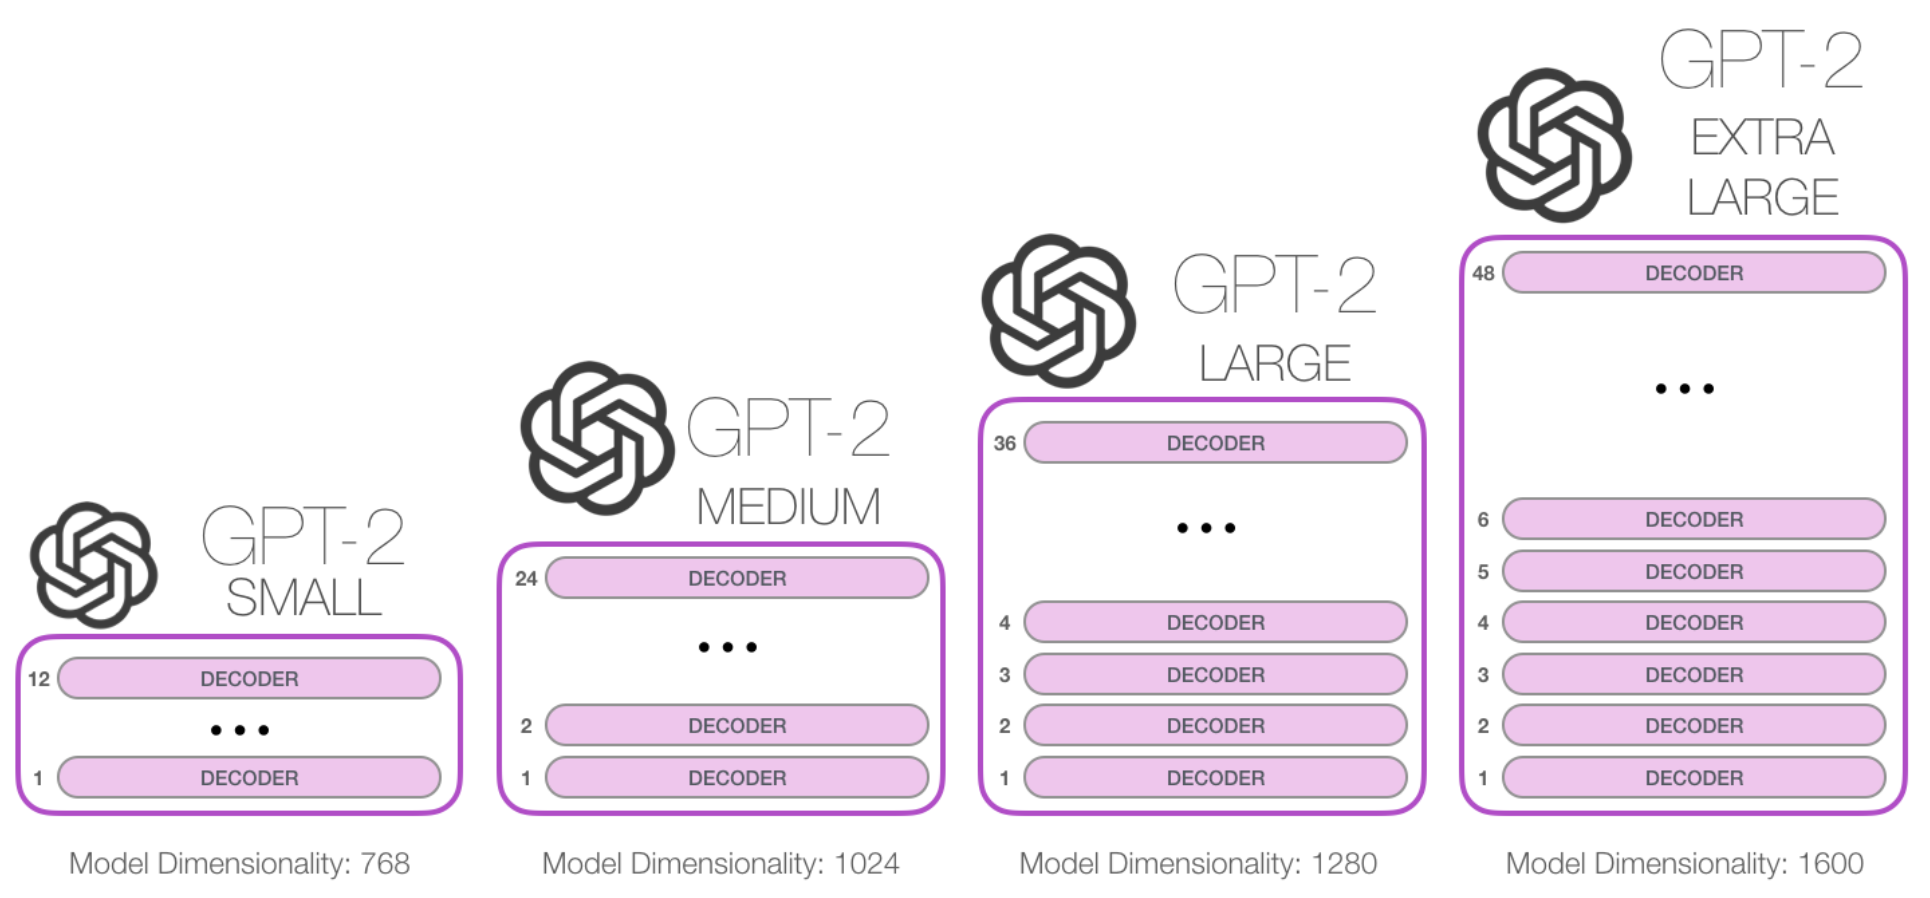
\includegraphics[width=0.85\textwidth]{figure/GPTModel}
    \caption{Possiamo vedere nell'immagine le varie tipologie di modelli di GPT-2, a seconda della dimensione del modello, si utilizzano più Decoder.}
    \label{fig:GPTModel}
\end{figure}

\subsection{Architettura e funzionamento}

GPT è un modello Transformer unidirezionale, ovvero genera una parola alla volta considerando solo il contesto precedente. Il principio fondamentale è l'Autoregressione: il modello predice la parola successiva $x_t$ data la sequenza delle parole precedenti $(x_1, x_2, ..., x_{t-1})$.

\subsubsection{Input e Tokenizzazione}

\begin{itemize}
    \item Il testo viene tokenizzato mediante una tecnica di tipo Byte-Pair Encoding (BPE);
    \item Ogni token viene convertito in un vettore di embedding;
    \item Viene aggiunto un \textit{positional embedding} per conservare l’informazione sull’ordine dei token;
    \item A differenza di BERT, non viene inserito alcun token \texttt{[CLS]} o \texttt{[SEP]}, poiché GPT non è progettato per la classificazione o il confronto fra frasi.
\end{itemize}

\subsubsection{Decoder e Self-Attention causale}

GPT utilizza unicamente blocchi Decoder del Transformer. Ogni blocco è composto da:
\begin{itemize}
    \item \textbf{Masked Self-Attention:} l'attenzione è limitata ai soli token precedenti mediante una \textit{causal mask}, impedendo al modello di vedere token futuri;
    \item \textbf{Feed-forward network:} applicato a ciascun token individualmente;
    \item \textbf{Layer normalization e Residual Connections:} analogamente al Transformer standard.
\end{itemize}

\subsubsection{Output e Generazione}

\begin{itemize}
    \item Il vettore finale associato all’ultimo token viene proiettato nello spazio vocabolario tramite una matrice di output;
    \item Viene applicata una softmax per ottenere una distribuzione di probabilità sulle parole successive;
    \item Il token con la probabilità più alta può essere selezionato (greedy), oppure campionato;
    \item Questo processo viene iterato per generare una sequenza coerente parola dopo parola.
\end{itemize}

\subsection{Scelta del Token successivo}
Una volta che viene effettuato il processo di analisi attraversando i Decoder, ciò che viene generato è un vettore in cui sono presenti diverse probabilità di preddizione relative alla parola successiva della nostra frase, per scegliere di quale parola si tratta ci sono varie modalità adottate:

\begin{itemize}
    \item\textbf{Argmax:} Scelto il token con probabilità massima;
    \item\textbf{Sampling:} Si estra un token a caso, seguendo la distribuzione di probabilità fornita;
    \item\textbf{Top-k sampling:} Si considerano solo i top-k token probabili, per poi selezionare il token fra questi;
    \item\textbf{Top-p nucleus sampling:} Vengono considerati solo i token la cui somma delle probabilità supera un valore $p$, per poi selezionare un token fra questi in maniera casuale;
    \item\textbf{Beam Search:} Vengono mantenute più sequenze candidate contemporaneamente, il costo computazionale è elevato;
\end{itemize}

\begin{Osservazione}
    L'argmax, è una specializzazione del Top-k sampling, dove il valore di k è unitario.
\end{Osservazione}

\subsection{Pretraining}

GPT viene pre-addestrato in modo non supervisionato su un ampio corpus testuale, ottimizzando la Cross-Entropy Loss per predire il token successivo:
\[
\mathcal{L} = -\sum_{t=1}^{T} \log P(x_t \mid x_1, ..., x_{t-1})
\]
Non vi è masking di token né predizione bidirezionale: il modello impara a generare testo in modo fluido e coerente, acquisendo conoscenza grammaticale, lessicale e semantica implicita.

\subsection{Utilizzo in downstream tasks}

GPT può essere adattato a compiti specifici in due modalità:

\begin{itemize}
    \item \textbf{Fine-tuning supervisionato:} il modello viene addestrato su dataset etichettati per compiti come classificazione, QA, traduzione, ecc\ldots (tipico in GPT-2);
    \item \textbf{Prompt-based learning:} grazie alla sua natura generativa, GPT può essere utilizzato in modalità \textit{zero-shot}, \textit{few-shot} o \textit{one-shot}, semplicemente modificando il prompt di input per adattarsi al task desiderato (approccio introdotto con GPT-3).
\end{itemize}

\begin{table}
    \centering
    \caption{Confronto tra BERT e GPT.}
    \begin{adjustbox}{width=\textwidth}
    \begin{tabular}{|l|c|c|}
    \hline
    \textbf{Caratteristica} & \textbf{BERT} & \textbf{GPT} \\
    \hline
    Architettura & Encoder Transformer & Decoder Transformer \\
    Direzionalità & Bidirezionale & Unidirezionale (autoregressivo) \\
    Obiettivo pretraining & MLM + NSP & Language Modeling \\
    Token speciali & [CLS], [SEP], [MASK] & Nessuno \\
    Uso principale & Comprensione del linguaggio & Generazione del linguaggio \\
    Modalità di utilizzo & Fine-tuning, feature extraction & Prompting, fine-tuning \\
    \hline
    \end{tabular}
    \end{adjustbox}
\end{table}
\section*{Approfondimenti}
\section{Varianti dei modelli Transformer}

Nel corso degli anni, numerose varianti dell’architettura Transformer sono state sviluppate per migliorarne l’efficienza, la generalizzazione e l’adattabilità a specifici compiti. Di seguito ne riportiamo alcuni:

\subsection{RoBERTa (Robustly Optimized BERT Approach)}

RoBERTa è una versione migliorata di BERT, introdotta da Facebook AI, che elimina l’obiettivo NSP, utilizza una maggiore quantità di dati e addestra il modello più a lungo. Le principali modifiche includono:
\begin{itemize}
    \item Rimozione del Next Sentence Prediction (NSP);
    \item Addestramento su batch più grandi e sequenze più lunghe;
    \item Dinamica del masking modificata ad ogni epoca.
\end{itemize}
RoBERTa ha mostrato prestazioni superiori a BERT in numerosi benchmark NLP.

\subsection{ALBERT (A Lite BERT)}

ALBERT propone un modello più leggero e scalabile mediante:
\begin{itemize}
    \item Condivisione dei pesi tra i layer;
    \item Fattorizzazione della matrice di embedding;
    \item Nuovo obiettivo di pretraining: \textit{Sentence Order Prediction (SOP)}.
\end{itemize}
Queste modifiche riducono drasticamente il numero di parametri, rendendo ALBERT più efficiente senza compromettere l’accuratezza.

\subsection{GPT-2, GPT-3, GPT-4 e oltre}

Le versioni successive della famiglia GPT (\textit{Generative Pre-trained Transformer}) hanno introdotto progressivi miglioramenti nella scala del modello, nella qualità dei dati di addestramento e nella stabilità dei processi di ottimizzazione. Ciascuna iterazione ha segnato un passo avanti verso la costruzione di modelli linguistici sempre più generali, multimodali e cognitivamente coerenti.

\begin{itemize}
    \item \textbf{GPT-2} (2019): rappresenta la prima versione di larga scala, con \textbf{1.5 miliardi di parametri} e addestramento su un vasto corpus di testi provenienti dal web. Mostrò per la prima volta la capacità di generare testi coerenti e grammaticalmente corretti su più paragrafi, introducendo il concetto di \textit{emergent behavior}, ovvero proprietà che nascono spontaneamente dall’aumento della dimensione del modello, senza modifiche architetturali. La sua pubblicazione fu inizialmente limitata per timori legati al potenziale uso improprio del modello;
    \item \textbf{GPT-3} (2020): ampliò drasticamente la scala, raggiungendo \textbf{175 miliardi di parametri}. È stato addestrato su dataset come \textit{Common Crawl}, \textit{BooksCorpus} e altre fonti ad alta qualità, con particolare attenzione alla diversità linguistica e stilistica. GPT-3 introdusse le capacità di \textbf{few-shot} e \textbf{zero-shot learning}, ossia la possibilità di risolvere compiti mai esplicitamente visti durante l’addestramento, semplicemente interpretando un prompt testuale. Questo segnò la transizione da modelli puramente linguistici a \textit{foundation models} in grado di generalizzare su differenti domini testuali;
    \item \textbf{GPT-4} (2023): rappresenta un’evoluzione non solo in termini di dimensione, ma anche di \textbf{qualità architetturale e robustezza contestuale}. È un modello \textbf{multimodale}, capace di elaborare sia testo che immagini, mostrando una comprensione più profonda delle relazioni semantiche e del ragionamento logico. Risulta più stabile rispetto alle versioni precedenti e presenta una migliore generalizzazione su compiti complessi, come la risoluzione di problemi matematici, la scrittura tecnica e la comprensione multimodale. Le sue prestazioni superano la soglia umana in numerosi benchmark, come MMLU, BIG-bench e HellaSwag, segnando un notevole salto qualitativo nella capacità di comprensione del linguaggio.
\end{itemize}

\subsection{ChatGPT e InstructGPT}

Con l’espansione della famiglia GPT, l’attenzione si è spostata dal semplice addestramento generativo verso la \textbf{messa a punto comportamentale} dei modelli, ossia la capacità di rispondere in modo utile, sicuro e coerente con le intenzioni umane.

\begin{itemize}
    \item \textbf{InstructGPT} (2022): è una versione di GPT-3 sottoposta a un processo di \textit{fine-tuning} mediante \textbf{Reinforcement Learning from Human Feedback} (RLHF). In questo approccio, annotatori umani valutano diverse risposte generate dal modello e assegnano un punteggio di preferenza. Un secondo modello, chiamato \textit{reward model}, apprende da queste valutazioni e guida il modello principale ad allinearsi meglio alle istruzioni fornite dall’utente. Il risultato è un comportamento più conforme alle aspettative umane, con risposte più pertinenti e un’evidente riduzione di bias e contenuti indesiderati.

    \item \textbf{ChatGPT} (fine 2022): nasce come applicazione conversazionale basata su InstructGPT e, successivamente, sulle versioni \textbf{GPT-3.5} e \textbf{GPT-4}. È progettato per generare risposte naturali, coerenti e contestualmente pertinenti, mantenendo la continuità del dialogo su più turni conversazionali. L’interfaccia di ChatGPT ha reso accessibile la potenza dei modelli linguistici a un vasto pubblico, promuovendo un’adozione senza precedenti dell’intelligenza artificiale generativa nel lavoro, nella ricerca e nella didattica.
\end{itemize}

\subsection{Evoluzioni Recenti: GPT-4 Turbo e GPT-4o}

Le iterazioni più recenti della famiglia GPT hanno ulteriormente migliorato la gestione del contesto, l’efficienza computazionale e la capacità multimodale del modello.

\begin{itemize}
    \item \textbf{GPT-4 Turbo} (2023): è una versione ottimizzata di GPT-4, progettata per offrire prestazioni equivalenti con un costo computazionale ridotto e una latenza inferiore. Supporta un contesto esteso fino a \textbf{128k token}, consentendo al modello di mantenere coerenza anche in testi di grande lunghezza o in conversazioni molto prolungate. È diventato il motore predefinito di ChatGPT a partire da fine 2023.

    \item \textbf{GPT-4o} (2024): segna una tappa fondamentale nello sviluppo dei modelli di linguaggio, introducendo la prima architettura \textbf{multimodale unificata} in grado di elaborare testo, immagini e audio all’interno di un singolo modello end-to-end. La sigla "o" sta per \textit{omni}, a indicare la capacità di operare su più modalità contemporaneamente. GPT-4o può percepire, comprendere e generare contenuti in tempo reale, con risposte vocali naturali e interpretazione visiva diretta, aprendo la strada a interfacce conversazionali sempre più immersive e interattive.
\end{itemize}

\subsection{GPT-5: Verso modelli sempre più generali e adattivi}

\textbf{GPT-5} rappresenta l’evoluzione più recente della serie \textit{Generative Pre-trained Transformer}, proseguendo la direzione tracciata da GPT-4o verso un'intelligenza realmente multimodale, interattiva e contestualmente consapevole. A differenza delle versioni precedenti, GPT-5 non si focalizza unicamente sull’aumento della scala, ma sulla \textbf{integrazione dinamica di memoria, ragionamento e apprendimento adattivo}. Le caratteristiche principali attese o già emerse includono:
\begin{itemize}
    \item Un’architettura \textbf{multimodale unificata}, capace di gestire testo, immagini, audio e video in un unico spazio di rappresentazione condiviso;
    \item \textbf{Memoria contestuale persistente}, per mantenere coerenza tra interazioni nel tempo e supportare apprendimento continuo;
    \item Forme avanzate di \textbf{ragionamento composizionale}, basate su strategie di \textit{chain-of-thought} e \textit{graph-of-thought};
    \item Un’ottimizzazione computazionale tramite \textbf{mixture-of-experts} e \textit{sparse attention}, che consente al modello di attivare solo i sotto-moduli necessari al compito corrente.
\end{itemize}

GPT-5 si configura dunque come un passo verso sistemi cognitivi più flessibili e adattivi, in cui la distinzione tra pre-addestramento e apprendimento continuo tende gradualmente a sfumare. L’obiettivo non è più soltanto generare testo, ma costruire un’intelligenza in grado di \textbf{interagire, ragionare e apprendere dal proprio contesto}.

\subsection{Verso la Prossima Generazione}

Le evoluzioni future dei modelli GPT e dei \textit{foundation models} in generale sembrano orientarsi verso tre direzioni principali:
\begin{enumerate}
    \item \textbf{Efficienza e sostenibilità:} riduzione dei costi computazionali mediante compressione dei parametri, quantizzazione e tecniche di \textit{sparse attention};
    \item \textbf{Memoria a lungo termine:} sviluppo di architetture dotate di memoria persistente, capaci di conservare conoscenze e aggiornarsi nel tempo;
    \item \textbf{Ragionamento multimodale e adattivo:} integrazione sempre più stretta tra linguaggio, visione, audio e interazione dinamica con l’ambiente.
\end{enumerate}

Questa traiettoria evidenzia come i modelli linguistici si stiano evolvendo da semplici predittori di testo a veri e propri \textbf{sistemi cognitivi generali}, capaci di apprendere, adattarsi e comprendere il mondo in maniera sempre più olistica e interattiva.


\subsection{Altri modelli noti}

\begin{itemize}
    \item \textbf{DistilBERT:} versione compressa di BERT, con il 40\% di parametri in meno e il 97\% delle performance;
    \item \textbf{ELECTRA:} introduce un pretraining discriminativo invece del classico MLM;
    \item \textbf{T5 (Text-to-Text Transfer Transformer):} unifica i compiti NLP in un’unica formulazione testuale.
\end{itemize}

\section{Applicazioni pratiche dei Transformer}

L’adattabilità dei modelli Transformer consente la loro applicazione in una vasta gamma di task di NLP, sia in modalità supervisionata (fine-tuning) che non supervisionata (prompt engineering):

\begin{itemize}
    \item \textbf{Classificazione testuale:} assegnazione di etichette a frasi, documenti, tweet, ecc. (es. analisi del sentiment);
    \item \textbf{Named Entity Recognition (NER):} identificazione di entità rilevanti nel testo (nomi, date, organizzazioni);
    \item \textbf{Risposta a domande (QA):} estrazione o generazione di risposte date una domanda e un contesto;
    \item \textbf{Traduzione automatica:} conversione da una lingua a un’altra (es. inglese → francese);
    \item \textbf{Generazione di testo:} produzione di frasi o paragrafi coerenti a partire da un prompt (storytelling, copywriting);
    \item \textbf{Riassunto automatico:} estrazione o generazione di versioni sintetiche di testi lunghi;
    \item \textbf{Conversational AI:} chatbot e assistenti virtuali, spesso costruiti su InstructGPT o ChatGPT;
    \item \textbf{Codice e programmazione:} generazione di codice (es. Codex), spiegazione di funzioni o completamento automatico.
\end{itemize}

\section{Evoluzione dei Transformer}

L’evoluzione dei modelli Transformer è stata caratterizzata da un rapido progresso sia in termini di architettura che di scala computazionale. Di seguito è riportata una timeline dei principali modelli:

\begin{itemize}
    \item \textbf{2017 – Transformer} \cite{vaswani2017attention}: introduzione dell’architettura self attentiva in "Attention is All You Need";
    \item \textbf{2018 – BERT} \cite{devlin2018bert}: encoder bidirezionale pre-addestrato con obiettivi MLM e NSP;
    \item \textbf{2019 – GPT-2} \cite{radford2019language}: modello autoregressivo di grandi dimensioni per generazione testuale;
    \item \textbf{2019 – RoBERTa} \cite{liu2019roberta}: ottimizzazione di BERT tramite addestramento più esteso e rimozione NSP;
    \item \textbf{2019 – DistilBERT} \cite{sanh2019distilbert}: distillazione di BERT per maggiore efficienza;
    \item \textbf{2020 – T5} \cite{raffel2020exploring}: approccio "text-to-text" per unificare i compiti NLP;
    \item \textbf{2020 – GPT-3} \cite{brown2020language}: 175 miliardi di parametri, abilità few-shot learning;
    \item \textbf{2020 – ELECTRA} \cite{clark2020electra}: discriminatore al posto di un tradizionale generatore;
    \item \textbf{2021 – InstructGPT} \cite{ouyang2022training}: RLHF per migliorare l’allineamento con le intenzioni umane;
    \item \textbf{2022 – ChatGPT}: versione ottimizzata per il dialogo basata su InstructGPT;
    \item \textbf{2023 – GPT-4}: modello multimodale con prestazioni avanzate in molti contesti;
    \item \textbf{2025 - GPT-5}: verso un'intelligenza realmente multimodale, interattiva e contestualmente consapevole.
\end{itemize}



